\section{Vertical Slice Demonstrator System}

\subsection{Overview and methodology}

\noindent The flexible architecture described above would allow early technical demonstration of the tracking trigger system, to identify possible real bottlenecks and find solutions, by studying, measuring and optimizing trigger latency, efficiency at different stages with hardware being developed.  This will also involve extensive simulation work, to guide the hardware implementation, as well as to compare the hardware testing results with that of expectations.  A possible Vertical Slice Demonstration setup is shown in Figure~\ref{fig:VS_TBench}, with each stage described below. For simplicity, we will often use the special configuration with eight Data Input Boards and four PRBs as an example to describe the concept. The architecture is very flexible to allow more advanced configurations, and we will decide which configuration to use for demonstration later.

\begin{figure}[ht!]
\centering
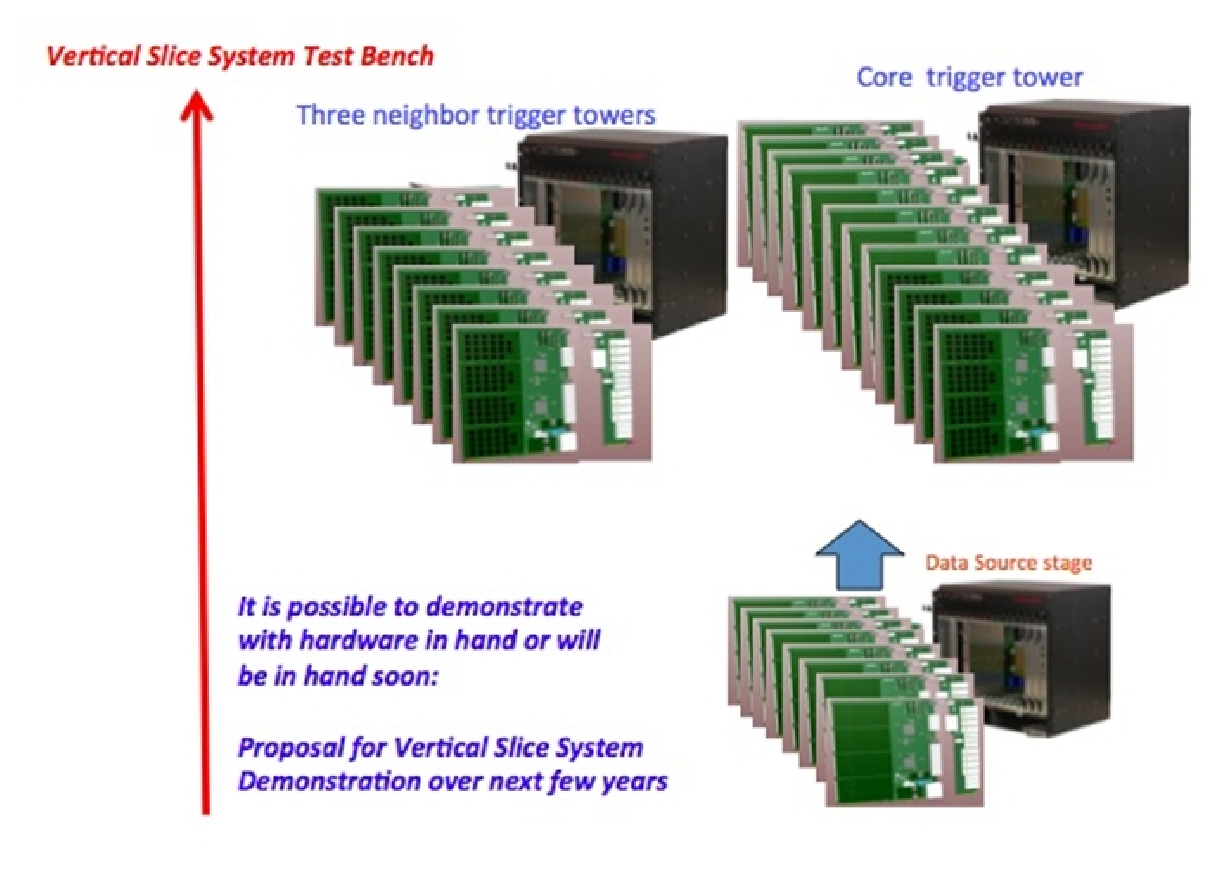
\includegraphics[width=0.7\columnwidth]{Plots/VS_TBench.eps}
\caption{Vertical slice test bench principle.}
\label{fig:VS_TBench}
\end{figure}

\subsection{Data Source Stage}

\noindent The Data Source stage's job is to mimic the upgraded Phase II outer-tracker running at the HL-LHC, to provide the data sources (about 300+ fibers/modules) for the trigger tower under study for the demonstration as if the data were coming from the real system with high luminosity (pile ups) collisions. Each fiber connection will transmit data with 3.2Gbps payload, in the same way as the actual module in the real system. The data will be derived from simulation and converted into hardware format, and stored in the on-board memory to be played out. 

\subsection{Data Input}

\noindent The Data Input Blade (DIB) is responsible for receiving data from the upstream detector electronics (or data source output) and transferring the data to the PRBs.  Up to ~40 fiber links will be received on each DIB.  These input links may terminate on the RTM or mezzanine cards.  Input fiber links are nominally 3.25Gb/s.  The Data Input Board will perform zero suppression, pack the found stubs into a new format and send them to the PRBs.  

\noindent Current estimate indicates that a baseline rate of about 200 stubs per event per trigger tower, which yields a data rate of roughly 256Gb/s (200 stubs*32bits/25ns) that goes into one trigger tower on average.  

\noindent As an example, in the configuration with eight DIBs and four PRBs, each PRB will be receiving 64 Gb/s stub data on average. Each of the eight DIBs in the shelf sends data to four PRBs in a round-robin, time multiplexed fashion.   Since data is sent to four PRBs these transfers can take place at a quarter of the input rate, or 8Gb/s.

\subsection{Pattern Recognition Board}

\noindent Again, using the special configuration above, each PRB will be receiving 64 Gb/s stub data on average.  While receiving the data and sending them to the mezzanine cards, each PRB will exchange data with the corresponding PRB (processing the same time slice) in the immediate neighbor (in other shelves or trigger towers) for data sharing in the overlap regions.  In this case, each PRB can use four 40Gb/s links (QSFP) for the connections in the eta and phi directions, and four 10Gb/s links (SFP+) can be used for data sharing in the "diagonal" directions (see Figure below for the shelf interconnections).
 
\noindent The PRB FPGA drives data received to the Pattern Recognition Mezzanine (PRM) boards, this can be done also in a 4x time multiplexed fashion.  The 4x time-multiplexed transfers from the PRB FPGA to the PRM would require a bandwidth of about 16Gb/s this way.  This also means that each PRM must contain all of the patterns for the trigger tower in this special configuration. 

\subsection{Pattern Recognition Mezzanine Card}

\noindent Each PRB supports four Pattern Recognition Mezzanine (PRM) boards.  These boards are based on the FMC standard and support high speed LVDS and SERDES connections to the PRB FPGA.  Each PRM will contain an FPGA, on board memory to act as Data Buffer, and an array of pattern recognition associative memory (PRAM) devices:  


\noindent In our example configuration, we need to support 16Gb/s between the PRB FPGA and the PRM.  This can be accomplished with an FPGA using three SERDES transceivers.  PRAM devices are attached to the FPGA using either a SERDES connection or multiple LVDS signal pairs.  The FPGA-PRAM channel bandwidth needs will be a fraction of the PRM input bandwidth, because only relevant stubs will be sent to the relevant AMchip covering the relevant regions of the trigger tower (see Figure below).

\noindent The PRM could be a logical successor to the test mezzanine card we have already designed. Future versions of the PRM will be designed to support different PRAM devices, such as AMCHIP0x (INFN) and the VPRAM0x (Fermilab). 

 
\subsection{PRAM and its Development}
  
\noindent As mentioned earlier, the CDF SVT-style Associative Memory chip (from now on we will call it PRAM, Pattern Recognition Associative Memory, to emphasis its purpose for HEP) is a departure beyond conventional CAMs. Like conventional CAMs, PRAMs store address patterns and look for matches between incoming hits and those addresses for a given detector layer. At this level, the match is expected to be either exact (Binary CAM) or partial (Ternary CAM) and an array of Match Flags is the typical output. A PRAM has an array of Match Flag Latches which capture and hold the results of the match until reset for the next event. As the hits from the various layers of the detector for the same event arrive, the PRAM is looking for more than simple matches from one candidate address to one or more stored address patterns. The PRAM organizes stored address patterns into roads, which are linked arrays of several stored address patterns from different detector layers.  Each stored address pattern in a road is from a different layer in the detector system and these linked arrays represent a path or road that a particle might traverse through the layers of the detector (hence the name "road"). The ultimate goal of the PRAM is to match real particle trajectories to those roads.  Like a conventional CAM, a PRAM flags a match when a candidate address matches a stored pattern address for a given detector layer. However, before the PRAM does anything with that match, it must find matches in all (or majority of) the elements (layers) that constitute a road.
 
\noindent It should be emphasized that compared to commercially available CAMs, such as Network Search Engine, the PRAM has the unique ability to search for correlations among input words received on different clock cycles.  This is essential for tracking trigger applications since the input words are the detector hits arriving from different layers at different times. They arrive at the chip without any specific timing correlation.  Each pattern has to store each fired layer until the pattern is matched or the event is fully processed. Even in the case of a level-1 trigger application, which is largely synchronous, this feature will still be important. One unique feature of this approach is that the pattern recognition of the event is done as soon as the last hit arrives, which makes the approach a promising candidate for L1 track trigger. However, the requirements for L1 track trigger application will be very different from that for L2, and the system interface of the chip has to be fully redesigned and the performance has to be optimized.
 
\noindent An upgraded PRAM chip (known as AMchip03 at CDF) was developed in 2005 by the CDF Italian collaborators~\cite{Ann-06}. The AMchip03 was implemented in 180nm technology using the Standard Cell approach and the number of patterns per chip increased by a factor of 40 over the previous version used at CDF, from 128 to 5,000. This chip, which runs at 40MHz, was used to upgrade the SVT system, where the total number of patterns has increased to more than 6 Million. However, in order to meet the challenges for the LHC high luminosity running, another increase in pattern density by two orders of magnitude will be required. The PRAM pattern density can be improved by optimizing the design in single-layer chips (2D), using custom cell designs with smaller feature size technology.  There is an R\&D effort by INFN using 65 nm technology to improve the standard cell based AMchip03 design for Atlas FTK application for L2 trigger (AMchip05 or 06). There is also an on-going R\&D effort at Fermilab using both conventional 2D and the emerging 3D technology to design future generation of PRAM chip~\cite{bib:VIP-11},\cite{bib:VIP-12} specifically for the L1 CMS tracking trigger needs (ProtoVIPRAM series). 

\subsection{Track Fitting stage} 

\noindent The traditional CDF SVT/FTK-style track fitting stage can be used to benchmark the performance of this stage. We are exploring other new approaches as well, such as Hough transform algorithm and tracklet-based algorithm. All track fitting algorithms should be implemented in FPGA on the PRMs, therefore they can be studied and compared directly using the same vertical slice demonstration setup. More detailed description of the two new approaches will become available in this section later. As a reference, the traditional SVT/FTK-style track fitting is described below~\cite{bib:FTK-10}.

\noindent For a region of detector sufficiently small, a linear approximation gives helix parameters close to those of full helical fit. In other words, for a road narrow enough that a helical fit can be replaced by a simple linear calculation.  Each of the 5 helix parameters (pi) can be calculated as the vector product of prestored constants (aij) and the hit coordinates (xj):   where N is the number of coordinates on the track, one for each SCT layer and two for each pixel layer.  Since there are more than 5 coordinates, there are additional linear equations that correspond to constraint equations:  , again where the constants are prestored.  There are (N - 5) such equations.  Each fi would be zero for perfect measurement; the sum of the squares of the fi's serves as the goodness of fit. 

\noindent This linear approximation gives near offline resolution for regions considerably wider than a single road.  A single set of constants will be used for each sector of the detector. The width of the sector at each silicon layer is the size of a physical detector module.  Per sector, 5�( N + 1) constants are needed for the helix parameters, and (N - 5)�( N + 1) constants are needed for the constraint equations.  The total number of fit constants (FC) per sector is thus N�(N + 1).

\noindent Will add some description here about CDF Gigafitter performance with FPGAs~\cite{bib:Ann-09}� etc. also with FTK most recent performance with modern FPGAs�

\subsection{Possible Work Breakdowns and Work Packages}

\noindent One of the main purposes of this document is to define the tracking trigger R\&D project and organize the efforts. In this section, we will describe possible work breakdowns and work packages for the Vertical Slice System Demonstration. The main work involved can be roughly divided into seven areas, and is shown in Figure z below. These seven areas can be future organized as seven Work Packages (see Figure z1)�.


\clearpage
